\Section
{فرمت داده‌ها}
{
	در کل، داده‌ها در چهار پوشه‌ی 
	\lr{raw}،
	\lr{clean}،
	\lr{sentencebroken}
	و
	\lr{wordbroken}
	قرار گرفته‌اند.
	
	\begin{center}
		\adjustbox{margin=1em, frame=1pt 1pt 1pt 1pt}{
			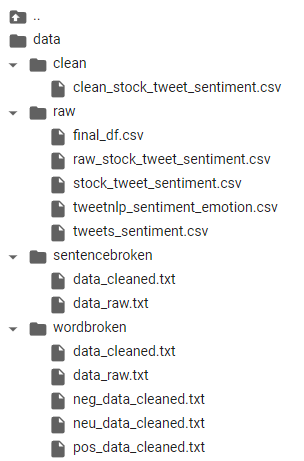
\includegraphics[scale=1]{Images/data_folder_structure.png}
		}
	\end{center}
	
	\begin{itemize}
		\item در پوشه 
		\lr{clean} 
		داده های تجمیع شده تمیز شده اند و روی آنها پیش پردازش صورت گرفته است و در ستون 
		\lr{tweet\_cleaned} 
		ذخیره شده اند.
		%%%%%%%%%%%%%%%%
		
		\item در پوشه 
		\lr{raw} 
		در صورتی که کد مربوط به 
		\lr{load} 
		کردن داده ها را اجرا کنید فایل های 
		\lr{csv} 
		مربوط به هر دیتاست در آن قرار می گیرند. به صورت پیش فرض این پوشه حاوی یک فایل 
		\lr{text}  
		است که در آن لینک دیتاست ها موجود است به همراه یک فایل اکسل 
		\lr{raw\_stock\_tweet\_sentiment.csv}
		دیتای خام چمع آوری شده از تمام دیتاست های ذکر شده است که شامل 120000 توییت می باشد
		%%%%%%%%%%%%%%%%
		
		\item در پوشه 
		\lr{sentencebroken} 
		داده های تمیز و خام بر اساس جمله 
		\lr{tokenize} 
		شده اند به صورتی که در هر خط این فایل ها یک جمله قرار گرفته است.
		%%%%%%%%%%%%%%%%
		
		\item در پوشه 
		\lr{wordbroken} 
		داده های تمیز و خام بر اساس کلمه 
		\lr{tokenize} 
		شده اند به صورتی که هر کلمه با یک 
		\lr{space} 
		از همدیگر جدا شده است
		همچنین توییت های موجود بر اساس برچسب نیز برحسب کلمه 
		\lr{tokenize} 
		شده اند
	\end{itemize}
	
}